\documentclass[11pt,a4paper,ngerman]{article}
\usepackage[bottom=2.5cm,top=2.5cm]{geometry} 
\usepackage{babel}
\usepackage[utf8]{inputenc} 
\usepackage[T1]{fontenc} 
\usepackage{ae} 
\usepackage{amssymb} 
\usepackage{amsmath}
\usepackage{amsthm} 
\usepackage{graphicx}
\usepackage{fancyhdr}
\usepackage{fancyref}
\usepackage{enumerate}
\usepackage{listings}
\usepackage{xcolor}
\usepackage{paralist}
\usepackage{tabularx}

\usepackage[pdftex, bookmarks=false, pdfstartview={FitH}, linkbordercolor=white]{hyperref}
\usepackage{fancyhdr}
\pagestyle{fancy}
\fancyhead[C]{Numerik I}
\fancyhead[L]{Übung 6}
\fancyhead[R]{SoSe 2013}
\fancyfoot{}
\fancyfoot[L]{}
\fancyfoot[C]{\thepage \hspace{1px} of \pageref{LastPage}}
\renewcommand{\footrulewidth}{0.5pt}
\renewcommand{\headrulewidth}{0.5pt}
\setlength{\parindent}{0pt} 
\setlength{\headheight}{0pt}

\date{Tutor : Christina Schulz}
\title{Übung 6}
\author{Max Wisniewski, Alexander Steen}


%%
%% Enviroments for proofs and lemmas
%%
\newtheorem{lemma}{\bfseries Claim}

\begin{document}

\lstset{language=Pascal, basicstyle=\ttfamily\fontsize{10pt}{10pt}\selectfont\upshape, commentstyle=\rmfamily\slshape, keywordstyle=\rmfamily\bfseries, breaklines=true, frame=single, xleftmargin=3mm, xrightmargin=3mm, tabsize=2, mathescape=true}

\renewcommand{\figurename}{Figure}

\maketitle
\thispagestyle{fancy}

%%%%%%%%%%%%%%%%%%%%%%%%%%%%%%
%% Aufgabe 1 %%%%%%%%%%%%%%%%
%%%%%%%%%%%%%%%%%%%%%%%%%%%%%%
\subsection*{Aufgabe 1}

Sei $S_\Delta^m$ der Raum der Splines $m$-ter Ordnung zum Gitter $\Delta = \{ t_0 , ..., t_n \}$.

Zeigen Sie
\begin{equation*}
    \dim S_\Delta^m = n + m.
\end{equation*}

\textbf{Beweis:}\\

Der Beweis steht schon fast vollständig im Skript.

Eine Funktion
\begin{equation*}
    f \in S_\Delta^m = \{ f \in C^{m-1}[a,b] \, | \, v|_{I_k} = p_k \in \mathcal{P}_m\}
\end{equation*}
wird, wie man sieht, durch $n$ Polynome beschrieben, die alle Grad $k$ haben.
Wir können $f$ also durch $n \cdot (m+1)$ Koeffizienten beschreiben.\\

Da die Funktion im Übergang $m-1$ fach stetig differenzierbar sein muss, gilt nach Übergangsbedingung,
dass $p_k^j(x_k) = p_{k+1}^(j)(x_k)$ für alle $0 \leq j < m$ und $0 \leq k < n$.\\

Wir verlieren nun für jede der Bedingungen einen Freiheitsgrad, da in den Punkten $t_k$ immer
gelten muss, dass die $i$-te Ableitung auf beiden angrenzenden Funktionen je eine Variable fest setzen
wird (wie wir bei der Interpolation vorher gesehen haben).

Pro Polynom ''verlieren'' wir so also $m$ Koeffizienten, die wir frei wählen können. Dies gilt nicht für
$t_0$ und $t_n$ da wir nicht auf die Rahmenbedingung zum Nachbarn achten müssen. Die restlichen
Koeffizienten können immer noch frei gewählt werden, da es sich beim Polynomring um einen Vektorraum handelt.

Folglich erhalten wir
\begin{equation*}
    \dim S_\Delta^m = \underbrace{n(m+1)}_\text{\#Mögliche Koeffizienten} - \underbrace{m(n-1)}_\text{stetig im Gitter} = n + m
\end{equation*}
\mbox{}\hfill$\square$

\subsection*{Aufgabe 2}

\subsubsection*{(a)}

Implementieren Sie eine Matlab Function für das Interpolieren/Approxmieren einer Funktion mit Kubischen Splines.\\

\textbf{Lösung:}\\
Die Funktion benutzt die Berechnungsvorschriften des Skriptes.
Für zwei Eingabelisten $[x_1,\ldots,x_k]$, $[y_1 = f(x_1),\ldots,y_k = f(x_k)]$ 
intepoliert die Funktion mittels kubischen Splines die Funktion $f$ und gibt
deren interpolierte Funktionswerte für die Eingabeliste $t = [t_1, \ldots, t_j]$
zurück.

\begin{lstlisting}[language=matlab,numbers=left]
\end{lstlisting}

\subsubsection*{(b)}

Testen Sie ihr Programm an der Funktion $f = \sqrt{5 + x}$ (WRONG).\\

\textbf{Lösung:}\\

tbd

\subsection*{Aufgabe 3}

Zeichnen Sie ihre Hand nach. Interpolieren Sie die gewählten Punkte mittels Kubischen Splines und natürlichen Randbedingungen
und interpolieren Sie es mittels pchip. Berechnen Sie es einmal über $x$ und einmal über $y$. Welchen unterschied
haben die beiden Verfahren.\\

\textbf{Lösung:}\\

Die Aufnahmepunkte wurden wie in der Aufgabe beschrieben erhoben und interpoliert. Abbildung~\ref{abb:1} zeigt die Interpolation der x-Koordinaten, Abbildung~\ref{abb:2} die Interpolation der y-Koordinaten; jeweils durch  die MATLAB-Funktion \texttt{pchip} und die MATLAB-Funktion \texttt{spline}\footnote{Unser Programm aus Aufgabe 2 wurde erst relativ spät fertig; darum haben wir schon vorher diese Aufgabe gelöst -- die Ergebnisse sollten aber die gleichen sein.}.
Leider war uns nicht klar, wie wir der Funktion \texttt{pchip} bzw. \texttt{spline} die ''natürlichen Randbedingungen'' übergeben sollen, da diese Funktion diese Eingabeparameter nicht vorsehen.

\begin{figure}[h]
\centering
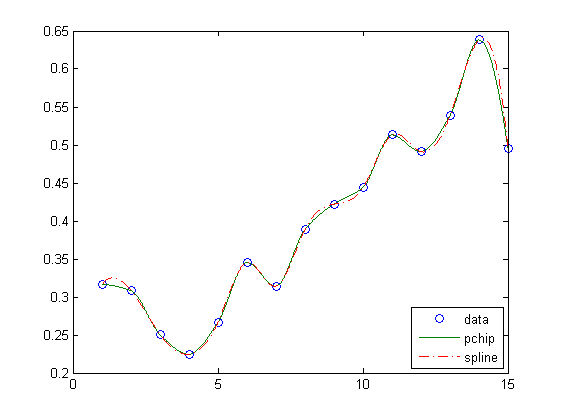
\includegraphics[width=0.8\textwidth]{plotX.png}
\caption{Interpolation der $x$-Koordinaten\label{abb:1}}
\end{figure}

\begin{figure}[h]
\centering
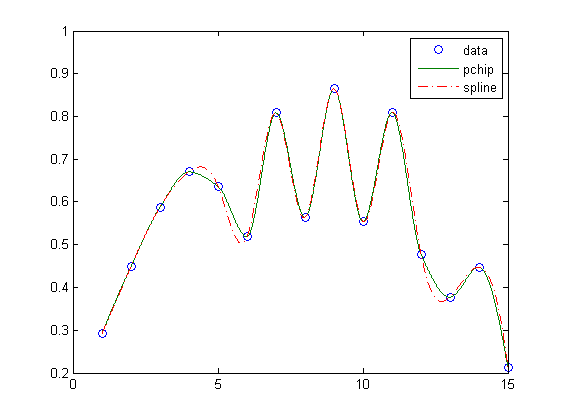
\includegraphics[width=0.8\textwidth]{plotY.png}
\caption{Interpolation der $y$-Koordinaten\label{abb:2}}
\end{figure}

\textbf{Beobachtungen}: Die Interpolation durch \texttt{spline} wirkt glatter bzw. ''geschmeidiger'',
macht also weniger starke bzw. enge Kurven. Die Kurven, die von \texttt{pchip} erzeugt werden, haben
weniger ''ausladende Schlaufen'', also keine kleine Oszillation um Datenpunkte.

\textbf{Erklärung}: Die beiden Methoden scheinen sich sehr stark zu ähneln. Der größte Unterschied ist,
dass \texttt{spline} die (stückweisen) Kurven so auswählt, dass die zweite Ableitung stetig ist.
Dies ist bei \texttt{pchip} nicht der Fall.
\label{LastPage}
\end{document}
